\section{DistSeal-inspired student: Direct top-10
resampling}\label{record-docs-watermarking-qualitative-text-latent-direct-topk-md-distseal-inspired-student-direct-top-10-resampling}

This is a fresh answer to the same prompt, not a rewrite.

Eight pairs selected by fixed test positions before inspecting detection
or quality outcomes. Undetected originals and unsuccessful attacks
remain included.

\begin{recordfigure}
\centering
\pandocbounded{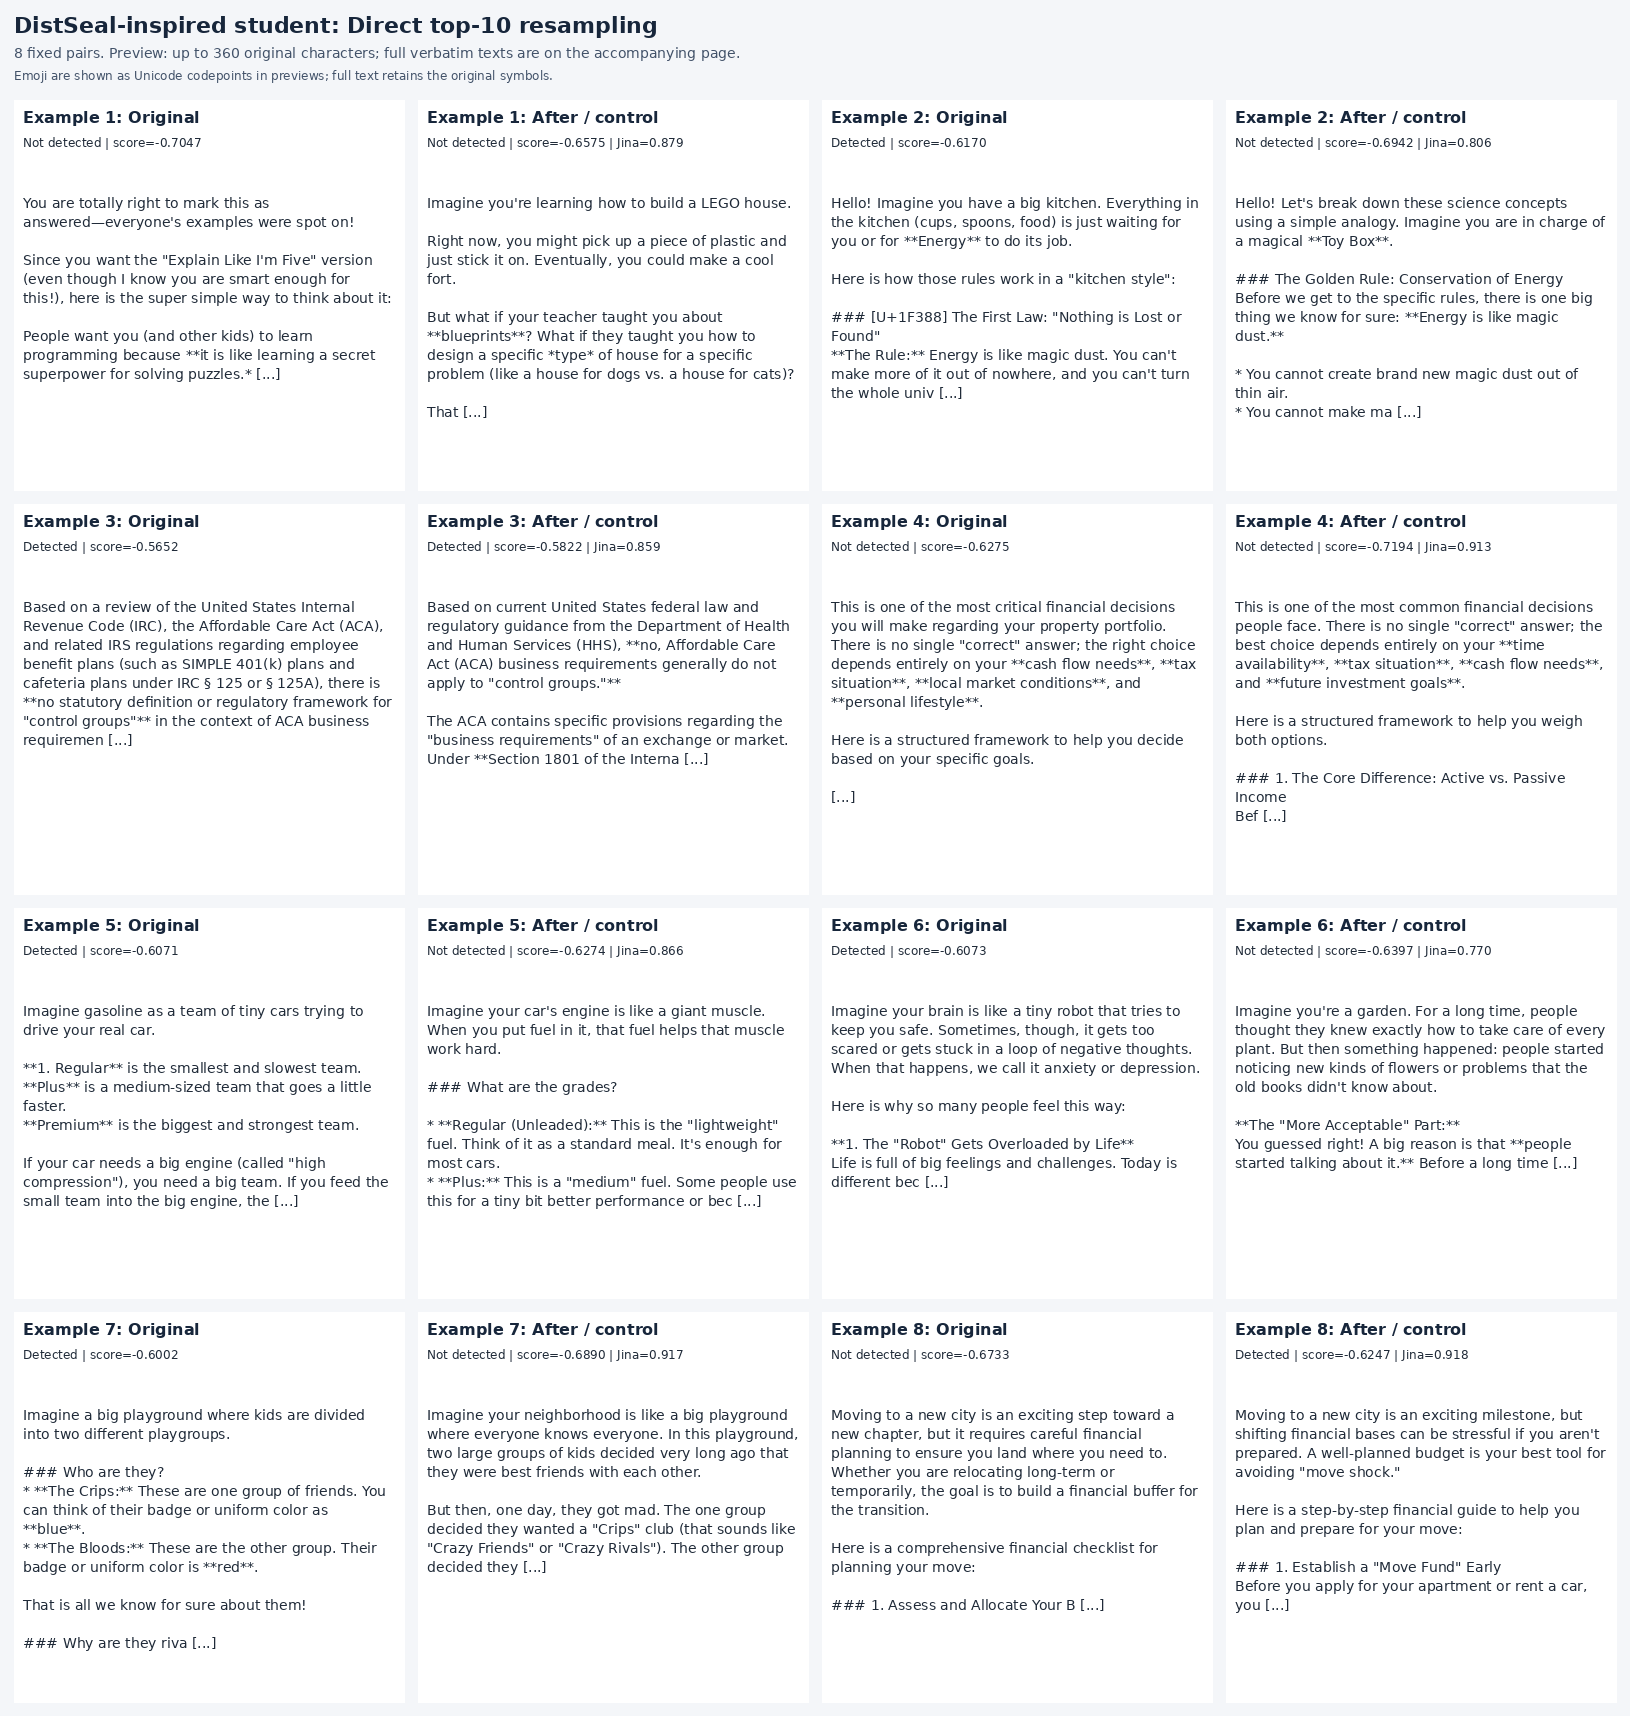
\includegraphics[keepaspectratio,alt={Sixteen-panel text preview}]{figures/text-latent-direct_topk.png}}
\caption{Sixteen-panel text preview}
\end{recordfigure}

The figure previews up to the first 360 original characters per
response; full texts below are unabridged. Emoji use Unicode codepoints
in the preview to avoid missing-glyph boxes. Owner scores and quality
metrics use full responses.

{\scriptsize\setlength{\tabcolsep}{3pt}\def\LTcaptype{none} % do not increment counter
\begin{longtable}[]{@{}
  >{\raggedright\arraybackslash}p{(\linewidth - 8\tabcolsep) * \real{0.2000}}
  >{\raggedright\arraybackslash}p{(\linewidth - 8\tabcolsep) * \real{0.2000}}
  >{\raggedright\arraybackslash}p{(\linewidth - 8\tabcolsep) * \real{0.2000}}
  >{\raggedright\arraybackslash}p{(\linewidth - 8\tabcolsep) * \real{0.2000}}
  >{\raggedright\arraybackslash}p{(\linewidth - 8\tabcolsep) * \real{0.2000}}@{}}
\toprule\noalign{}
\begin{minipage}[b]{\linewidth}\raggedright
Example
\end{minipage} & \begin{minipage}[b]{\linewidth}\raggedright
Test position
\end{minipage} & \begin{minipage}[b]{\linewidth}\raggedright
Before
\end{minipage} & \begin{minipage}[b]{\linewidth}\raggedright
After
\end{minipage} & \begin{minipage}[b]{\linewidth}\raggedright
Jina
\end{minipage} \\
\midrule\noalign{}
\endhead
\bottomrule\noalign{}
\endlastfoot
1 & 0 & Not detected \textbar{} score=-0.7047 & Not detected \textbar{}
score=-0.6575 & 0.8789 \\
2 & 32 & Detected \textbar{} score=-0.6170 & Not detected \textbar{}
score=-0.6942 & 0.8060 \\
3 & 64 & Detected \textbar{} score=-0.5652 & Detected \textbar{}
score=-0.5822 & 0.8586 \\
4 & 96 & Not detected \textbar{} score=-0.6275 & Not detected \textbar{}
score=-0.7194 & 0.9135 \\
5 & 128 & Detected \textbar{} score=-0.6071 & Not detected \textbar{}
score=-0.6274 & 0.8657 \\
6 & 160 & Detected \textbar{} score=-0.6073 & Not detected \textbar{}
score=-0.6397 & 0.7704 \\
7 & 192 & Detected \textbar{} score=-0.6002 & Not detected \textbar{}
score=-0.6890 & 0.9168 \\
8 & 224 & Not detected \textbar{} score=-0.6733 & Detected \textbar{}
score=-0.6247 & 0.9181 \\
\end{longtable}
}

\subsection{Example 1: test position
0}\label{record-docs-watermarking-qualitative-text-latent-direct-topk-md-example-1-test-position-0}

Prompt ID:
\texttt{\seqsplit{eb41610306c3726e0a74a6888b55bc82ea505683f3fe908e286b197665852b84}}.

\textbf{Question / prompt}

\begin{Verbatim}
Why do people want programming taught in elementary / high schools ? I know absolutely nothing about programming . EDIT : I 'm marking this as answered . Thanks to everyone who replied ! Explain like I'm five.
\end{Verbatim}

\textbf{Original watermarked-model output}

\begin{Verbatim}
You are totally right to mark this as answered[U+2014]everyone's examples were spot on!

Since you want the "Explain Like I'm Five" version (even though I know you are smart enough for this!), here is the super simple way to think about it:

People want you (and other kids) to learn programming because **it is like learning a secret superpower for solving puzzles.**

Here is why:

1.  **It teaches you how computers think.**
    Computers don't "feel" or "guess." They only follow rules. Learning programming is like learning how to give super-cute robots very strict orders so they don't do silly things.

2.  **It helps kids learn other subjects faster.**
    Imagine trying to learn English by reading books. Then imagine trying to learn math by writing video games. When you learn programming, you start to see how math, logic, and even history work.

3.  **The biggest reason?
\end{Verbatim}

\textbf{After / alternative output}

\begin{Verbatim}
Imagine you're learning how to build a LEGO house.

Right now, you might pick up a piece of plastic and just stick it on. Eventually, you could make a cool fort.

But what if your teacher taught you about **blueprints**? What if they taught you how to design a specific *type* of house for a specific problem (like a house for dogs vs. a house for cats)?

That's what learning programming is like!

People want you to learn it for these three simple reasons:

1.  **It's a super-power for solving problems.**
    Instead of just playing with one piece of plastic or building one LEGO set, knowing how to program means you can use your "computer brain" to tell machines how to build *anything*. You could help clean up your room without a robot, or draw a picture of your cat.

2.  **You need to understand "why" things work.**
    If you know how computers work
\end{Verbatim}

Recorded diagnostics:
\texttt{\seqsplit{\{"mistral\_perplexity": 8.5\}}}.

\subsection{Example 2: test position
32}\label{record-docs-watermarking-qualitative-text-latent-direct-topk-md-example-2-test-position-32}

Prompt ID:
\texttt{\seqsplit{55ce85cdcf38f9b189c667d07ffb34cc5bd73600e98a2987c721e3a8c166c343}}.

\textbf{Question / prompt}

\begin{Verbatim}
Thermodynamics Could someone explain to me the first , and second laws of thermodynamics , and conservation of energy ? Explain like I'm five.
\end{Verbatim}

\textbf{Original watermarked-model output}

\begin{Verbatim}
Hello! Imagine you have a big kitchen. Everything in the kitchen (cups, spoons, food) is just waiting for you or for **Energy** to do its job.

Here is how those rules work in a "kitchen style":

### [U+1F388] The First Law: "Nothing is Lost or Found"
**The Rule:** Energy is like magic dust. You can't make more of it out of nowhere, and you can't turn the whole universe inside out and disappear. The total amount of energy is always exactly the same.

**[U+1F449] "Explain like I'm five":**
Imagine a coin. You don't spend coins faster than you find them.
- If you find **$10** on the ground.
- And you buy a **$5** candy.
- You now have **$5** of energy left.

Even if you drop the candy and your feet get dirty or you eat the candy,
\end{Verbatim}

\textbf{After / alternative output}

\begin{Verbatim}
Hello! Let's break down these science concepts using a simple analogy. Imagine you are in charge of a magical **Toy Box**.

### The Golden Rule: Conservation of Energy
Before we get to the specific rules, there is one big thing we know for sure: **Energy is like magic dust.**

*   You cannot create brand new magic dust out of thin air.
*   You cannot make magic dust disappear into nothing.

You can only turn the magic dust from one form into another (like turning a toy car into heat by rolling it fast). This is called the **Law of Conservation of Energy**.

Think of a **battery** in a remote control. The battery holds "energy dust." When you turn on the remote, the dust turns into electricity to power the lights. But where did the dust go? It didn't vanish! Maybe some of it turned into a tiny bit of heat in the buttons.

### The First Law: Energy Can't Be Magic
\end{Verbatim}

Recorded diagnostics:
\texttt{\seqsplit{\{"mistral\_perplexity": 7.5\}}}.

\subsection{Example 3: test position
64}\label{record-docs-watermarking-qualitative-text-latent-direct-topk-md-example-3-test-position-64}

Prompt ID:
\texttt{\seqsplit{3cd335e45281f1d50700d93f931fc20b2f8fef24b7084ab3b583f745105137b1}}.

\textbf{Question / prompt}

\begin{Verbatim}
Do Affordable Care Act business requirements apply to “control groups?”
\end{Verbatim}

\textbf{Original watermarked-model output}

\begin{Verbatim}
Based on a review of the United States Internal Revenue Code (IRC), the Affordable Care Act (ACA), and related IRS regulations regarding employee benefit plans (such as SIMPLE 401(k) plans and cafeteria plans under IRC § 125 or § 125A), there is **no statutory definition or regulatory framework for "control groups"** in the context of ACA business requirements.

The terms "control groups" and "control vs. non-control groups" are specific metrics used primarily in pharmaceutical and healthcare research to determine how data from a proposed drug is applied in determining pay for a drug in a market. Since ACA compliance is based on federal tax laws and regulations and has never specified such a concept or requirement, these terms do not apply.

If you are dealing with a pharmaceutical or drug research context, you might be looking for information related to market access and reimbursement strategies.

**Answer:**
No. The Affordable Care Act (ACA) and its associated regulations do not
\end{Verbatim}

\textbf{After / alternative output}

\begin{Verbatim}
Based on current United States federal law and regulatory guidance from the Department of Health and Human Services (HHS), **no, Affordable Care Act (ACA) business requirements generally do not apply to "control groups."**

The ACA contains specific provisions regarding the "business requirements" of an exchange or market. Under **Section 1801 of the Internal Revenue Code (26 U.S.C. § 2601)**, the definition of a "business" is critical. The law explicitly defines "business" for the purposes of this section in **26 U.S.C. § 2601(d)(3)(A)** as:

> "the term 'business' shall include a for-profit corporation, partnership or sole proprietorship and **any other entity that is engaged in a trade or business or for profit**."

However, more importantly for your specific question regarding control groups and market access (specifically **Section 1801(b)** of the
\end{Verbatim}

Recorded diagnostics:
\texttt{\seqsplit{\{"mistral\_perplexity": 6.40625\}}}.

\subsection{Example 4: test position
96}\label{record-docs-watermarking-qualitative-text-latent-direct-topk-md-example-4-test-position-96}

Prompt ID:
\texttt{\seqsplit{28bb030845669613f0466940878780ef6fe5149ef4223cb7b87d0ce22e4d30b3}}.

\textbf{Question / prompt}

\begin{Verbatim}
Should I sell a 2nd home, or rent it out?
\end{Verbatim}

\textbf{Original watermarked-model output}

\begin{Verbatim}
This is one of the most critical financial decisions you will make regarding your property portfolio. There is no single "correct" answer; the right choice depends entirely on your **cash flow needs**, **tax situation**, **local market conditions**, and **personal lifestyle**.

Here is a structured framework to help you decide based on your specific goals.

### 1. The Core Trade-off: Liquidity vs. Asset Appreciation
Before diving into the details, understand the fundamental difference in how these strategies work:

*   **Selling:** You realize your profit or loss immediately. You convert the asset into cash (liquidity). Your goal here is usually cash flow or moving on from the property.
*   **Renting:** You forgo immediate profit for potential long-term appreciation and tax benefits (like Schedule E depreciation in the US). You keep the asset on your balance sheet.

### 2. Key Factors to Consider

#### A. Your Immediate Financial Needs
*   **
\end{Verbatim}

\textbf{After / alternative output}

\begin{Verbatim}
This is one of the most common financial decisions people face. There is no single "correct" answer; the best choice depends entirely on your **time availability**, **tax situation**, **cash flow needs**, and **future investment goals**.

Here is a structured framework to help you weigh both options.

### 1. The Core Difference: Active vs. Passive Income
Before diving into the specifics, understand that this decision defines your relationship with the property for the next 10–20 years.

| Feature | Rent It Out | Sell It |
| :--- | :--- | :--- |
| **Income Type** | Passive (or semi-passive) monthly income. | One-time lump sum. |
| **Effort** | High. Requires tenant management, maintenance, and compliance with landlord laws. | Moderate. Requires staging, marketing, and closing process (1–3 months). |
| **Cash Flow** | Positive monthly flow (Rent -
\end{Verbatim}

Recorded diagnostics:
\texttt{\seqsplit{\{"mistral\_perplexity": 5.53125\}}}.

\subsection{Example 5: test position
128}\label{record-docs-watermarking-qualitative-text-latent-direct-topk-md-example-5-test-position-128}

Prompt ID:
\texttt{\seqsplit{ba7280e98e1cd80ce7a2ecb56c06dcc0cccae5126f2c806c9c87951a5c32a351}}.

\textbf{Question / prompt}

\begin{Verbatim}
Can somebody explain what different grades of gasoline mean ( regular , plus , premium ) and why I should use anything but regular ? Edit : Thanks guys , despite getting up to 10 year old vocabulary , you 've answered my question very well Explain like I'm five.
\end{Verbatim}

\textbf{Original watermarked-model output}

\begin{Verbatim}
Imagine gasoline as a team of tiny cars trying to drive your real car.

**1. Regular** is the smallest and slowest team.
**Plus** is a medium-sized team that goes a little faster.
**Premium** is the biggest and strongest team.

If your car needs a big engine (called "high compression"), you need a big team. If you feed the small team into the big engine, they can't pull hard enough. The engine would start popping or "knocking" like a crowbar hitting a rock.

You shouldn't use anything but Regular unless:
- Your car is old or very small (like an old bike), or
- Your car came with a specific note from the owner saying "Use Premium for Best Performance"

So, you'd stick with Regular for those older or smaller cars.

If your car needs a big engine, you need a big team. If you feed the small team into the big engine, they can
\end{Verbatim}

\textbf{After / alternative output}

\begin{Verbatim}
Imagine your car's engine is like a giant muscle. When you put fuel in it, that fuel helps that muscle work hard.

### What are the grades?

*   **Regular (Unleaded):** This is the "lightweight" fuel. Think of it as a standard meal. It's enough for most cars.
*   **Plus:** This is a "medium" fuel. Some people use this for a tiny bit better performance or because they live in an area where regular gas is very cheap or hard to find.
*   **Premium:** This is the "heavyweight" fuel. Think of it as a special meal made for very big or very strong muscles.

### Why should you use anything but regular?

Here is the secret: **You should almost never use anything but regular.**

Here is why:

1.  **Your car doesn't want it:** Most cars come with a fuel filter that only lets a specific size of fuel through.
\end{Verbatim}

Recorded diagnostics:
\texttt{\seqsplit{\{"mistral\_perplexity": 6.28125\}}}.

\subsection{Example 6: test position
160}\label{record-docs-watermarking-qualitative-text-latent-direct-topk-md-example-6-test-position-160}

Prompt ID:
\texttt{\seqsplit{b1f1f19f49ef99f6892eb93dd82a9582e1819ca3b02645f3d8eb75d6851036e9}}.

\textbf{Question / prompt}

\begin{Verbatim}
Howcome anxiety and depression are so common ? Is it something to do with society and lifestyles or how children are raised ? Or is it simply because it 's more acceptable to talk about it which means it 's more easily diagnosed ? Explain like I'm five.
\end{Verbatim}

\textbf{Original watermarked-model output}

\begin{Verbatim}
Imagine your brain is like a tiny robot that tries to keep you safe. Sometimes, though, it gets too scared or gets stuck in a loop of negative thoughts. When that happens, we call it anxiety or depression.

Here is why so many people feel this way:

**1. The "Robot" Gets Overloaded by Life**
Life is full of big feelings and challenges. Today is different because we are on the Internet! We get worried about school or our friendships. Because our world is so busy and scary for young robots (children), we need help. That is why doctors are finding these problems more often.

**2. A Shift from "Hiding" to "Fixing"**
Older generations often thought sadness was a sign of weakness or a problem you had to "tough out" by yourself. They would just leave you alone or ignore it. But now, people are taught to talk about their feelings. When you tell a friend or doctor about how
\end{Verbatim}

\textbf{After / alternative output}

\begin{Verbatim}
Imagine you're a garden. For a long time, people thought they knew exactly how to take care of every plant. But then something happened: people started noticing new kinds of flowers or problems that the old books didn't know about.

**The "More Acceptable" Part:**
You guessed right! A big reason is that **people started talking about it.** Before a long time ago, it was very hard for families to say their children were sick or had "bad feelings." They might have thought it was just being lazy or not trying hard enough.

Now, doctors and parents are better at noticing when someone is sad or worried for too long. Because we talk about it more, we find it more often.

**But is that ALL there is?**
Think about the weather in your garden. Sometimes the sky gets very dark or very hot.

1.  **Hard Work (Lifestyles):** Many people are running very fast all day. They have many jobs to do
\end{Verbatim}

Recorded diagnostics:
\texttt{\seqsplit{\{"mistral\_perplexity": 12.1875\}}}.

\subsection{Example 7: test position
192}\label{record-docs-watermarking-qualitative-text-latent-direct-topk-md-example-7-test-position-192}

Prompt ID:
\texttt{\seqsplit{413d7314d50fdc47803344b8bf0b0e9291797c0b2e2296b73b1d78a212e69257}}.

\textbf{Question / prompt}

\begin{Verbatim}
What is the difference between the Crips and the Bloods . Why are they rivals ? What do each do ? Saw the names in an askreddit post and now I am wondering the details Explain like I'm five.
\end{Verbatim}

\textbf{Original watermarked-model output}

\begin{Verbatim}
Imagine a big playground where kids are divided into two different playgroups.

### Who are they?
*   **The Crips:** These are one group of friends. You can think of their badge or uniform color as **blue**.
*   **The Bloods:** These are the other group. Their badge or uniform color is **red**.

That is all we know for sure about them!

### Why are they rivals?
The main reason they fight is a game of **"Third Place."**

Imagine a race where everyone is trying to be number one.
*   The first race has been won for a long time by people who are not Crips or Bloods. (Let's call them "Others").
*   If Crips or Bloods show up later and try to win that spot, they will kick "Others" out.

Now, "Others" are gone. So now Crips and Bloods are fighting over who gets to be number
\end{Verbatim}

\textbf{After / alternative output}

\begin{Verbatim}
Imagine your neighborhood is like a big playground where everyone knows everyone. In this playground, two large groups of kids decided very long ago that they were best friends with each other.

But then, one day, they got mad. The one group decided they wanted a "Crips" club (that sounds like "Crazy Friends" or "Crazy Rivals"). The other group decided they wanted a "Bloods" club.

**Why are they rivals?**
Imagine they decided they were going to be enemies because of a silly argument about colors or a song that one group liked and the other didn't. They swore they would fight each other.

*   **The Crips** decided they would wear **Black** clothes.
*   **The Bloods** decided they would wear **Red** clothes.

**What do each "do"?**
For a long time, people used to think that these groups were just playing a game.
*   Sometimes kids from
\end{Verbatim}

Recorded diagnostics:
\texttt{\seqsplit{\{"mistral\_perplexity": 7.75\}}}.

\subsection{Example 8: test position
224}\label{record-docs-watermarking-qualitative-text-latent-direct-topk-md-example-8-test-position-224}

Prompt ID:
\texttt{\seqsplit{3bca8fb40ea23a3b89f55baf6f1df768cadc687ae8a97bbbfc98c7db825a44ac}}.

\textbf{Question / prompt}

\begin{Verbatim}
I am moving to a new city. How do I plan and prepare - financially - for the move?
\end{Verbatim}

\textbf{Original watermarked-model output}

\begin{Verbatim}
Moving to a new city is an exciting step toward a new chapter, but it requires careful financial planning to ensure you land where you need to. Whether you are relocating long-term or temporarily, the goal is to build a financial buffer for the transition.

Here is a comprehensive financial checklist for planning your move:

### 1. Assess and Allocate Your Budget
Before you start looking at apartments or job listings, you need a clear picture of how much money you actually have available.

*   **Calculate Upfront Moving Costs**: Estimate one-time expenses. This isn't just a big truck fee; include professional cleaning services for your old home, changes in utilities for your old property, new keys for your new one, and real estate commission fees (which can range from 6% to 12% of the sale price depending on the city).
*   **Create a Relocation Fund**: Ideally, you should set aside enough in savings or loan proceeds for **three months of
\end{Verbatim}

\textbf{After / alternative output}

\begin{Verbatim}
Moving to a new city is an exciting milestone, but shifting financial bases can be stressful if you aren't prepared. A well-planned budget is your best tool for avoiding "move shock."

Here is a step-by-step financial guide to help you plan and prepare for your move:

### 1. Establish a "Move Fund" Early
Before you apply for your apartment or rent a car, you should ideally save a specific amount for moving expenses. Do not let this money get spent on groceries or bills until the move is finalized.
*   **Target Amount**: Estimate 30–40% of your total move costs upfront.
*   **Sources**: Consider using emergency funds, tax refunds, or a dedicated high-yield savings account.

### 2. Map Your Costs to the Timeline
Moving costs often surprise people who only look at the "big" costs (trucking, movers). Break them down chronologically:

**Pre-Move Expenses (1
\end{Verbatim}

Recorded diagnostics:
\texttt{\seqsplit{\{"mistral\_perplexity": 7.625\}}}.

\href{records/docs/watermarking/text.tex}{Text metrics} \textbar{}
\href{../docs/watermarking/README.md}{Report overview}
